\begin{SingleSpace}
\chapter{The Atmospheric Circulation of Tidally Locked Exoplanets}\label{ch:lava-planets}
%\addcontentsline{toc}{chapter}{\nameref{ch:lava-planets}}

% \vspace{0.5cm}
% \chapterprecishere{``One face is forever sunlit, and one forever dark, and only the planet's slow liberation gives the twilight zone a semblance of seasons.''\par\raggedleft--- \textup{Stanley G. Weinbaum}, The Lotus Eaters}
\end{SingleSpace}
% \vspace{0.5cm}

This chapter reviews relevant work on the global circulation of tidally locked planets. It discusses the discovery and characterisation of exoplanets, focusing on the measurements that are relevant to their atmospheric composition and dynamics. It reviews the formation of a tidally locked state, and the resulting atmospheric circulation, then introduces the ``lava planet'' 55 Cancri e.

%SECTION 1 -- EXOPLANETS
\section{Exoplanets}

Exoplanets are planets orbiting stars other than our Sun. Several thousand exoplanets have been discovered, showing a large variety of planetary types including many unlike anything in the Solar System. I will use the word ``exoplanet'' when discussing specific planets or issues relating to observations, and ``planet'' in a more general context. It is possible to characterise the atmospheres of some exoplanets, measuring their composition or even the effects of their global circulation.

Figure \ref{fig:review-planet-population} shows all the exoplanets from the NASA Exoplanet Archive\footnote{\url{exoplanetarchive.ipac.caltech.edu}} for which radii and orbital periods were available at the time of writing. It shows several distinct populations. The first divide is between the rocky planets in the lower part below approximately $R = 3 R_{E}$ and the gaseous planets above this. The division between these two classes is by no means exact \citep{perryman2018exoplanet}. In the lower left-hand corner are the terrestrial tidally locked planets considered in this thesis, including the hot ``lava planets'' discussed later. The rocky planets with longer orbital periods are more similar to the inner planets in the Solar System. At larger radii are the ``super-Earths'', and then the gaseous ``mini-Neptunes' -- again, there is no exact division between the populations. At the top of the plot are the gas giants. The hot Jupiters on the left have short orbital periods, and provide the best observations of the atmospheres of tidally locked planets.

% . Above these, in the centre of the plot, we have the rocky ``Super-Earths' with radii around $2 R_{E}$, and the larger gaseous ``Mini-Neptunes''. The exact division between these populations is not clear. At the top of the plot are the Jupiter-sized gas giants. On the left are the short-period ``hot Jupiters'', which are generally well suited for characterisation via transit observations. On the right are the cooler gas giants, which are better suited to detection by radial velocity or direct imaging techniques.

\begin{figure}
  \centering
    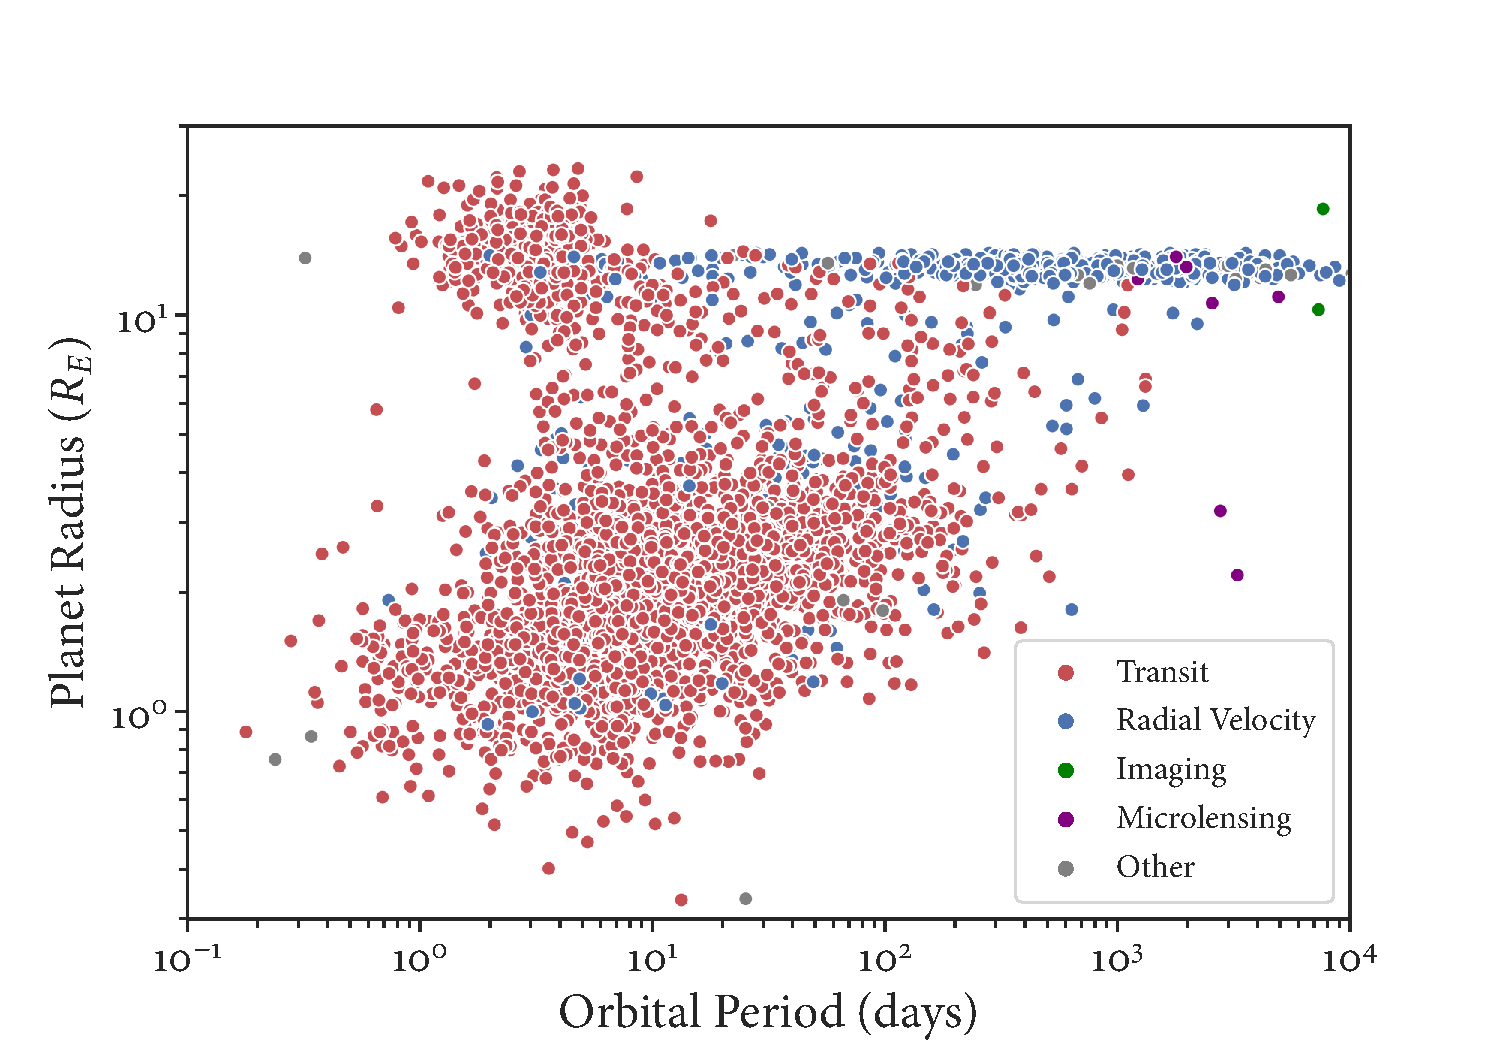
\includegraphics[width=1.0\textwidth]{figures/lit-review/planet-population.pdf}
    \caption{The population of known exoplanets plotted by planetary radius and orbital period, labelled by discovery method. The discovery methods are biased towards planets with particular properties.}\label{fig:review-planet-population}
\end{figure}


%SUBSECTION -- DISCOVERY
\subsection{Discovering Exoplanets}

Most exoplanets discovered to date have been found using either a ``radial velocity'' method or a ``transit'' method \citep{perryman2018exoplanet}. In the radial velocity (Doppler spectroscopy) method, the motion of a star around its common centre of mass with an orbiting planet is detected by measuring the Doppler-shift of emission lines of the star. The magnitude and period of this motion give the period of the planet's orbit, and a lower limit on its mass, owing to the degeneracy between the mass and the inclination in their effect on the signal.

In the transit method, an observer measures the reduction in flux from the star when the planet crosses the line of sight from the observer to the star (its ``primary transit''). The time between successive transits gives the orbital period of the planet, and the depth of the transit gives the radius of the planet at the wavelength observed. Combining the mass and period from a radial velocity measurement with the radius and period from a transit observation also gives the density and equilibrium temperature of the planet, which are vital for understanding planetary composition and important for atmospheric modelling.

Figure \ref{fig:review-planet-population} shows how different discovery methods are biased towards the detection of different types of planet. The red dots show planets discovered by the transit method, which are currently the most common due to the success of the \textit{Kepler} telescope. These planets are clustered to the left of the plot, as transits are more likely to be detected for close-in planets in short-period orbits, which reduce the flux from their star more strongly when they transit. The blue dots show planets detected by the radial velocity method, which produces stronger signals for higher-mass planets like the gas giants at the top of the plot.

The planets shown in green were detected by direct imaging, in which the light from their host star is blocked with a coronagraph and the planet is directly observed. This is currently only possible for young, large, self-luminous planets orbiting far from their star, so these planets are found to the top right of the plot. Direct imaging will become possible for more planets in the coming decade \citep{perryman2018exoplanet}.

%SUBSECTION -- CHARACTERISATION
\subsection{Characterising Exoplanets}

The atmospheres of exoplanets can be characterised with transmission and emission spectroscopy. Transmission spectroscopy measures the spectrum of light from the host star that passes through the atmosphere of the exoplanet as it transits. Measuring the depth of the transit at different wavelengths gives the radius of the planet and its atmosphere at those wavelengths, which depends on the opacity of the atmosphere. This allows the absorption spectrum of the gases in the atmosphere to be reconstructed, which can then be used to estimate the composition of the atmosphere \citep{tsiaras2016detection}.



Emission spectroscopy measures the spectrum of the thermal emission of the planet and its atmosphere. Hotter planets are better suited to this method as they emit more strongly at thermal wavelengths. The thermal emission depends on the composition of the atmosphere and its thermal structure, meaning that it can be used to reconstruct the vertical structure of the atmosphere \citep{stevenson2014thermal}.

Features of the atmospheric circulation of exoplanets are starting to be measured. The bulk wind speed of the atmosphere of an exoplanet can be measured via the Doppler-shift of absorption lines in its transmission spectrum \citep{louden2015spatially, brogi2016rotation}. Phase curve observations of the thermal emission of an exoplanet over its whole orbit have been used to infer the atmospheric circulation on hot Jupiters \citep{zellem2014hd209, parmentier2017handbook}, which I will discuss in more detail later.


%SECTION 2 -- TIDALLY LOCKED PLANETS
\section{Tidally Locked Planets}

An asynchronously rotating planet like the Earth has a different rotation period (1 day) to its orbital period (1 year). A synchronously rotating, or ``tidally locked'', planet has the same rotation period as its orbital period. This means that it always presents the same face to its host star, so it has a permanent day-side and a permanent night-side. I explained previously that planets orbiting close to their star are more likely to be detected, and are better suited to atmospheric characterisation. This section will show that these close-in planets are more likely to be tidally locked. This means that tidally locked planets should make up many of the best targets for atmospheric observations \citep{crossfield2015observations}.



%SUBSECTION -- DYNAMICS
\subsection{Formation}

All planets are affected by tidal stress due to their gravitational interaction with their host star. At the centre of mass of the planet, the gravitational force exactly balances the centrifugal force. The gravitational attraction is stronger than the centrifugal force for the part of the planet closest to the star, and the opposite is true for the part of the planet further from the star. This produces a stress that elongates the planet along the axis between it and the star. If the planet is not tidally locked, the long axis of the resulting ellipse will rotate away from this axis, and the stress will deform the planet further. This continual deformation removes rotational kinetic energy from the planet, until it reaches a tidally locked state where the long axis of the ellipsoid points towards the star permanently and no more energy is dissipated. Stable spin-orbit resonances are also possible, such as the 3:2 resonant orbit of Mercury, so not all planets affected by these stresses will reach a 1:1 tidally locked state.

The gravitational tidal stress acting on a planet is $\Sigma=2 G M_{*} / r^{3}$, where $M_{*}$ is the mass of the star and $r$ is the distance between the planet and the star \citep{pierrehumbert2018review}. The cubic dependence on $r$ makes the tidal locking timescale very sensitive to the semi-major axis. \citet{pierrehumbert2018review} estimate the time for a planet to become tidally locked to be:

\begin{equation}
  t_{\mathrm{lock}}=3.01 \times 10^{8} \frac{\rho \Omega_{0} r^{6}}{M_{*}^{2}} \frac{Q}{k_{2}},
\end{equation}

where $r$ is the mean orbital distance in AU, $\rho$ is the mean density of the planet in units of Earth density, and $\Omega$ is the angular velocity of the planet in units of Earth angular velocity. $Q$ corresponds to the effect of the dissipation of energy from tidal stresses \citep{goldreich1966q}, and $k_{2}$ is the Love number, which depends on the rigidity of the planet \citep{barnes2017tidal}. \citet{pierrehumbert2018review} use values for Earth and Venus to estimate the ratio for a generic terrestrial planet as $Q/k_{2} \approx 1000$.

 \citet{pierrehumbert2018review} use this formula to estimate that the rocky Earth-sized planet Trappist-1d would become tidally locked in 4000 years, assuming that it forms with the same initial angular velocity as Earth. By the same approximation, the super-Earth lava planet 55 Cancri e would take 6 years to reach this state. These short timescales suggest that the planets are very likely to be tidally locked. It is less clear whether planets with estimated tidal locking timescales of millions or billions of years will actually have reached this state.

\citet{leconte2015asynchronous} showed how atmospheric thermal tides oppose the gravitational tides discussed above, and slow the progress towards tidal locking. Thermal tides are caused by the thermal inertia of the atmosphere creating an excess of mass in the atmosphere  which lags behind the substellar point of an asynchronously rotating planet. The gravitational pull of the star on this mass excess produces a torque on the atmosphere, which acts on the planet in the opposite direction to the torque from the gravitational tide. Figure \ref{fig:review-leconte-tl} shows that this could inhibit tidal locking on Earth-mass planets. This effect would not be important for hot Jupiters, or the lava planets investigated in this thesis, but it is worth remembering that the simple estimate of a ``tidal locking timescale'' is not the whole story for many planets.

\begin{figure}
  \centering
  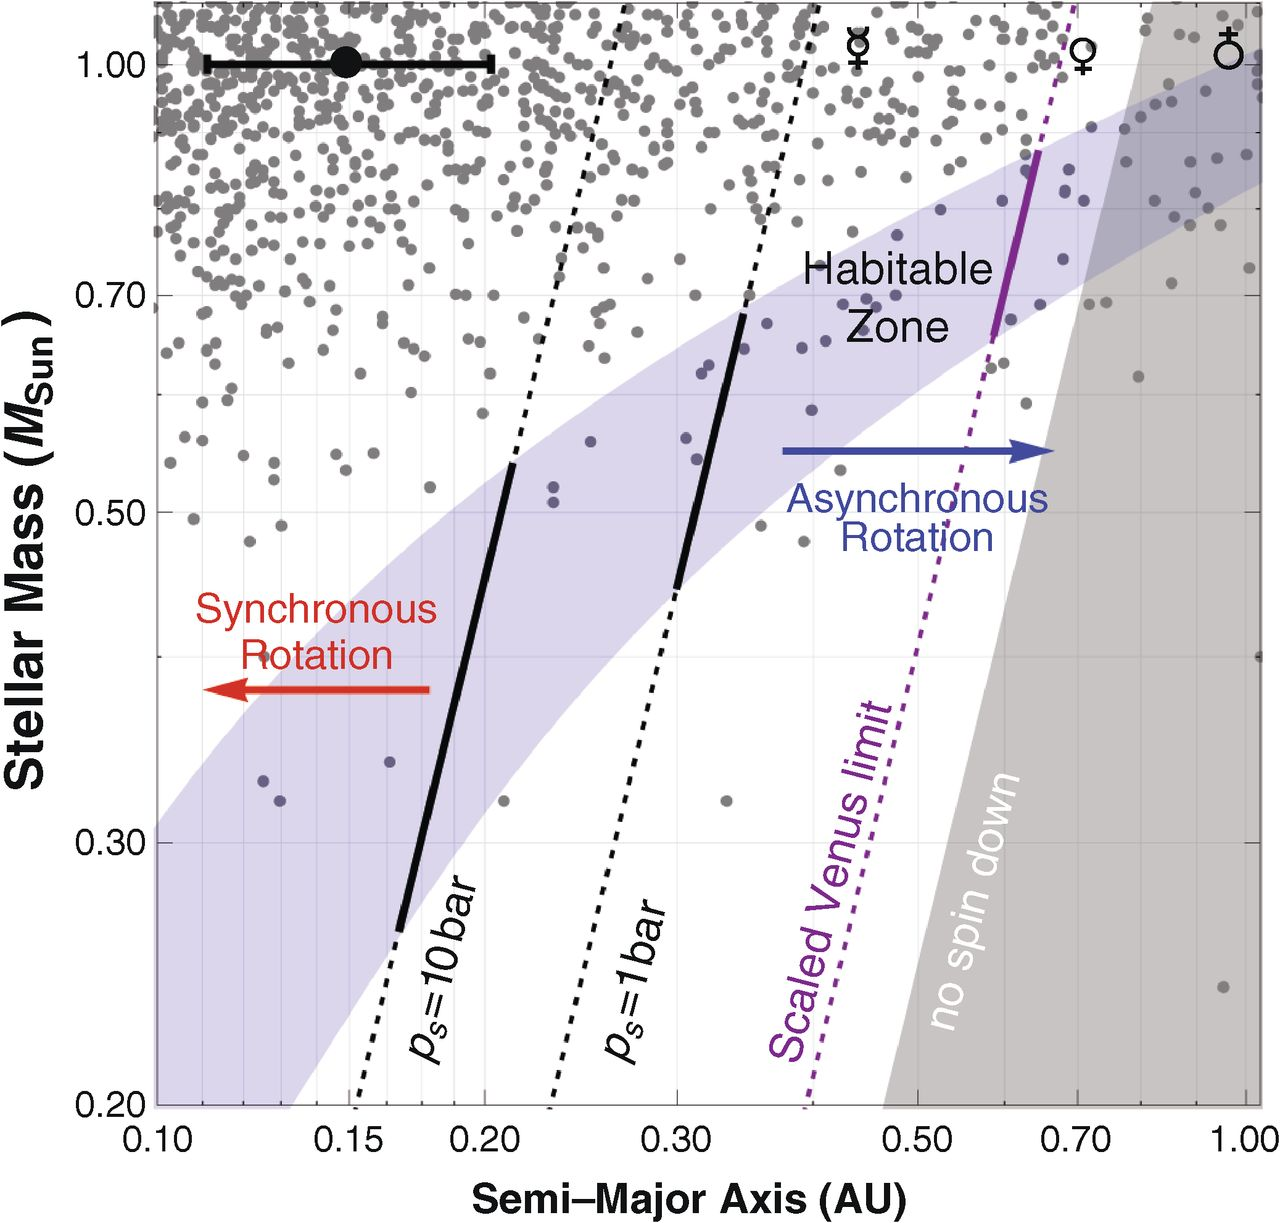
\includegraphics[width=0.6\textwidth]{figures/lit-review/leconte-tl.jpg}
\caption{A parameter space of stellar mass versus semi-major axis for discovered exoplanets, with lines showing the regions expected to have tidally locked planets with atmospheres of different thicknesses, from \citet{leconte2015asynchronous}. The thermal tide of the atmosphere may prevent Earth-like planets from become tidally locked.}\label{fig:review-leconte-tl}
\end{figure}


%SUBSECTION -- 55 Cancri system
\subsection{Lava Planets and 55 Cancri e}

Chapters \ref{ch:linking-climate-55cnce} and \ref{ch:clouds-lava-planets} investigate the atmospheric dynamics of ``lava planets''. These are hot rocky planets with a partially or fully molten surface, known as a ``magma ocean''. Lava planets are well suited to atmospheric observations due to their high temperatures and proximity to their stars, so are useful case studies for understanding the atmospheric dynamics of tidally locked planets.

55 Cancri e is the best-characterised example of a lava planet. It is a super-Earth with radius $1.95\ \mathrm{R_{E}}$ and orbital period 0.737 days \citep{crida201855cnce}. \citet{mcarthur2004detection} first detected the planet via the radial velocity method with an incorrect period of 2.808 days. \citet{dawson2010radial} showed that this period was due to spurious aliasing caused by gaps in the observations and corrected the period. It is expected to be tidally locked due to the short tidal locking timescale estimated above, and the observations of \citet{demory201655cnce}.

 % \citet{madhusudhan2012possible} used interior models constrained by mass and radius measurements of 55 Cancri e to suggest that its interior is carbon-rich. More recently, \citet{dorn2018new} suggested that it is one of a class of similar Super-Earths with a lower interior density than the Earth, with no core.

 \citet{demory201155cnce} and \citet{winn2011super} detected transits of the planet at infrared and visible wavelengths, opening the possibility of atmospheric characterisation.  \citet{demory2015variability} measured variable day-side thermal emission from 55 Cancri e over eight secondary eclipses, and suggested that this could be due to large-scale changes on the surface caused by strong tidal interactions with the star. \citet{tsiaras2016detection} reported the detection of an atmosphere with the WFC3 instrument on the Hubble Space Telescope, which appeared to be hydrogen-rich with a possible detection of HCN. The possibility of observing the composition of an atmosphere of the planet with emission spectroscopy has been explored by \citet{miguel2018observability} and \citet{ito2015theoretical}, who simulated a variety of spectra of potential atmospheres of different compositions and thicknesses.



%SUBSECTION -- PHASE CURVE
\subsection{A Thermal Phase Curve of 55 Cancri e}


\begin{figure}
  \centering
  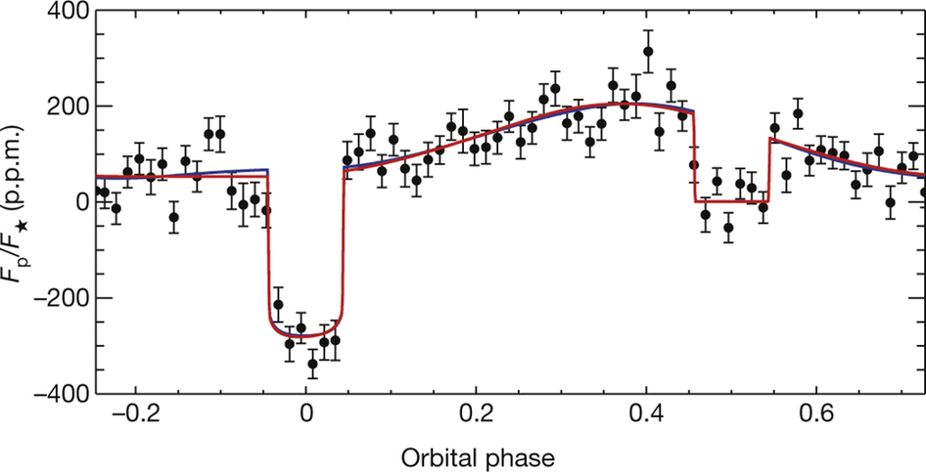
\includegraphics[width=0.7\textwidth]{figures/linking-climate-55cnce/demory-phase-curve.jpg}
\caption{The thermal phase curve observed in the \SI{4.5}{\micro\metre} \textit{Spitzer} bandpass by \citet{demory201655cnce}, showing an offset of the maximum flux from the secondary eclipse (the second dip), corresponding to a hot-spot shift possibly caused by atmospheric circulation. Reproduced from \citet{demory201655cnce} with permission.}\label{fig:review-demory-phase-curve}
\end{figure}


A ``phase curve'' is the radiation received from a planet over one complete orbit of its star. They contain information about how the emission or albedo of the planet varies with longitude, showing features such as day-night temperature differences. Phase curves measured at thermal wavelengths correspond to the radiating temperature of the planet or its atmosphere, so show features such as day-night temperature contrasts on tidally locked planets. Phase curves measured at optical wavelengths show the light from the host star reflected by the planet, so can show how the albedo of the planet varies due to heterogeneous features such as clouds \citep{parmentier2016transitions,parmentier2017handbook}. The phase curve has no latitudinal resolution, as the flux at any orbital phase only depends on the longitude at which the planet is observed. Techniques such as ``eclipse mapping'' can also retrieve latitudinal information, but require stronger emission from the planet \citep{majeau20122dmap}.

\begin{figure}
  \centering
  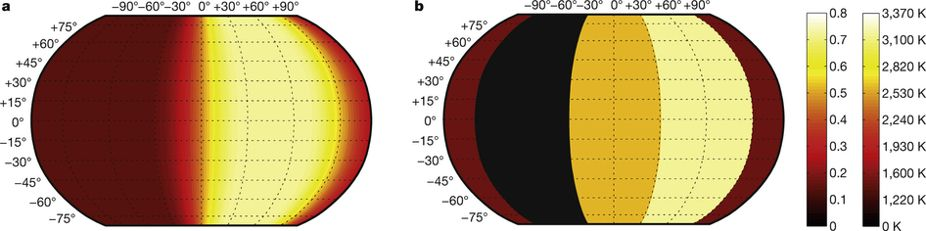
\includegraphics[width=0.95\textwidth]{figures/linking-climate-55cnce/demory-temp-maps.jpg}
\caption{The temperature map reconstructed by \citet{demory201655cnce} from the phase curve in Figure \ref{fig:demory-phase-curve}, showing a hot-spot shift of \ang{41}, a day-side temperature of \SI[separate-uncertainty = true]{2700(270)}{\kelvin}, and a night-side temperature of \SI[separate-uncertainty = true]{1380(400)}{\kelvin}. Reproduced from \citet{demory201655cnce} with permission.}\label{fig:review-demory-temp-maps}
\end{figure}

Phase curves are especially relevant to the atmospheric dynamics investigated in this thesis as the longitudinal variation of temperature on a planet can depend strongly on its global circulation. Figure \ref{fig:review-demory-phase-curve} shows the thermal phase curve of 55 Cancri e measured by \citet{demory201655cnce} using the \SI{4.5}{\micro\metre} channel of the \textit{Spitzer} space telescope. Figure \ref{fig:review-demory-temp-maps} shows the map of brightness temperature inferred from this phase curve. The phase curve implies a night-side temperature of \SI{1300}{\kelvin}, implying a significant warming of the night-side by atmospheric heat transport. It also shows a hot-spot shifted \SI{41}{\degree} east of the substellar point, which would be the hottest part without any atmospheric circulation. This hot-spot shift is similar to the phase shift in the optical phase curve measured by \citet{dragomir2012most} with the \textit{MOST} space telescope, which set an upper limit of 0.6 on its geometric albedo.

\citet{angelo201755cnce} analysed this phase curve using a similar 1D energy balance model to \citet{zhang2017dynamics}. They tuned the planetary Bond albedo, atmospheric surface pressure, heat redistribution efficiency, and greenhouse effect in this model, to match the observed phase curve. The parameters that fit best were a surface pressure of \SI{1.4}{\bar} and a heat redistribution efficiency of 1.47 (the ratio of radiative to advective timescales).

% The thermal phase curves of 55 Cancri e and other tidally locked planets motivated the work in this thesis to understand the atmospheric dynamics of tidally locked planets, and to simulate their observable consequences.



%SUBSECTION -- DYNAMICS
\section{Atmospheric Dynamics}

This section discusses current models of the dynamics of exoplanet atmospheres, and the theory of their global circulation. It introduces the concept of superrotation, which is a key part of the circulation of tidally locked planets.

\subsection{Numerical Atmospheric Models}

A General Circulation Model (GCM) is a three-dimensional fluid dynamical model of the atmosphere or the ocean of a planet, or both. They have been used to model the Earth, other planets in the Solar Systems, and are now used to simulate a wide variety of exoplanet atmospheres, often closely matching observations \citep{heng2015review, arcangeli2019climate}. GCMs typically consist of a dynamical core coupled to a representation of physical forcing such as radiative transfer or convective adjustment. The physics modelled in a GCM can range from very simple parameterisations capturing key processes \citep{held1994proposal} to highly detailed models of interacting clouds, radiative transfer, or other small-scale processes \citep{lines2018simulating, drummond2018observable}.

The GCM Exo-FMS used in this thesis based on the GFDL Flexible Modelling System\footnote{\url{gfdl.noaa.gov/fms/}} and the associated cubed-sphere dynamical core\footnote{\url{gfdl.noaa.gov/cubed-sphere-quickstart/}} \citep{ding2016convection, pierrehumbert2016dynamics, hammond2017climate, hammond2018wavemean}. Appendix \ref{ap:exo-fms} outlines the overall structure of the model, the dynamical core and associated grids, and the physics modules that can be swapped in and out of the model.

In the field of exoplanet studies, GCMs have perhaps been applied most successfully to modelling the atmospheres of hot Jupiters \citep{showman2002atmospheric, mayne2014unified, parmentier2016transitions, amundsen2016hd209, mayne2017hotjupiter}. Terrestrial planets have also been modelled to suggest potential circulation regimes or stable climate states \citep{merlis2010atmospheric, showman2012review, boutle2017proxima, noda2017circulation}. Other classes of exoplanet such as super-Earths or mini-Neptunes have been modelled in varying levels of detail \citep{carone2015regimes, charnay20153d, heng2015review}.


\subsection{Superrotation}\label{sec:superrotation}

Superrotation refers to a state where an atmosphere has more angular momentum than the solid planet below it. There are different ways of defining this mathematically -- I will use the definition of \citet{read1986super}, which defines superrotation as a positive ``superrotation index'', corresponding to an excess of atmospheric angular momentum over solid-body rotation at the equator. The local superrotation index is:

\begin{equation}
  s=\frac{m}{\Omega a^{2}}-1,
\end{equation}

where $\Omega$ is the planetary angular velocity, $a$ is the radius, and the specific angular momentum $m$ is:

\begin{equation}
 m=a \cos \phi(\Omega a \cos \phi+u),
\end{equation}

where $\phi$ is the latitude and $u$ is the local zonal velocity. An atmosphere with an ``ideal'' meridional circulation would homogenise the angular momentum of the equatorial surface in its upper branch, so the local superrotation index would be zero at all latitudes in that layer. The meridional circulation does not achieve this in reality (as on the Earth) and the superrotation index will be negative in most places \citep{read2018superrotation}. A process transporting angular momentum towards the equator, such as the stationary waves on tidally locked planets that produce an equatorial jet \citep{showman2011superrotation}, can produce an excess of angular momentum. This gives a positive local superrotation index at the equator.

The global superrotation index is a mass-weighted integral of the local superrotation index, and corresponds to a global measure of the magnitude of superrotation in the atmosphere:

\begin{equation}
  S_{m}=\frac{\iiint \rho m \mathrm{d} V}{\iiint \rho \Omega a^{2} \cos ^{2} \phi\ \mathrm{d} V}-1,
\end{equation}

where $\rho$ is the local density, and $\iiint \mathrm{d} V$ is an integral over the total volume of the atmosphere. Hide's Theorem states that the local $s$ and global $S_{m}$ cannot be positive anywhere without up-gradient angular momentum fluxes \citep{hide1969dynamics}. Superrotation is found in the atmosphere of Earth and other planets in the Solar System such as Venus and Titan \citep{laraia2015superrotation, read2018superrotation, sugimoto2019fully}. In this thesis, eastward angular momentum is transported towards the equators of tidally locked planetary atmospheres, producing a superrotating equatorial jet \citep{showman2011superrotation}.

\subsection{Dynamics of Tidally Locked Atmospheres}

The atmospheres of tidally locked planets are forced by their star in a very different way to the planets in the Solar System. The main source of atmospheric dynamics is the strong contrast in heating and cooling between the day-side and the night-side. This could be expected to drive an isotropic flow from the substellar point on the day-side to the antistellar point on the night-side, which can sometimes appear in simulations of very slowly rotating or strongly damped atmospheres \citep{pierrehumbert2018review, arcangeli2019climate}. In more realistic cases with faster rotation, the day-night forcing excites stationary waves that pump eastward momentum towards the equator, producing a superrotating jet that transports heat from the day-side to the night-side \citep{showman2011superrotation}. I will investigate the formation of this zonal flow in Chapter \ref{ch:eqm-zonal-flow}.

This equatorial superrotation was predicted by GCM simulations of terrestrial and gaseous tidally locked planets before its effects were observed \citep{joshi1997tidally, showman2002atmospheric}. These simulations predicted that the jet would shift the hottest part of the planet to the east of the substellar point, which was found to be true in thermal phase curves measured for many hot Jupiters \citep{parmentier2017handbook}. Figure \ref{fig:review-ar_mediumT_10day} shows a typical global temperature map from a simulation of a tidally locked planet, with the hot-spot shifted east of the substellar point. This shift was initially thought to be caused by pure advection of heat by the flow, but \citet{tsai2014three} showed that the eastward jet could shift the stationary waves excited by the day-night forcing eastwards, producing the hot-spot shift. \citet{perez2013atmospheric} also showed that the wave timescale is more important to this shift than the advective timescale of a hot Jupiter. I will discuss this in more detail in Chapter \ref{ch:wave-mean-flow}, and will show how a latitudinally sheared equatorial jet produces the global circulation pattern and hot-spot shift.

\begin{figure}
  \centering
  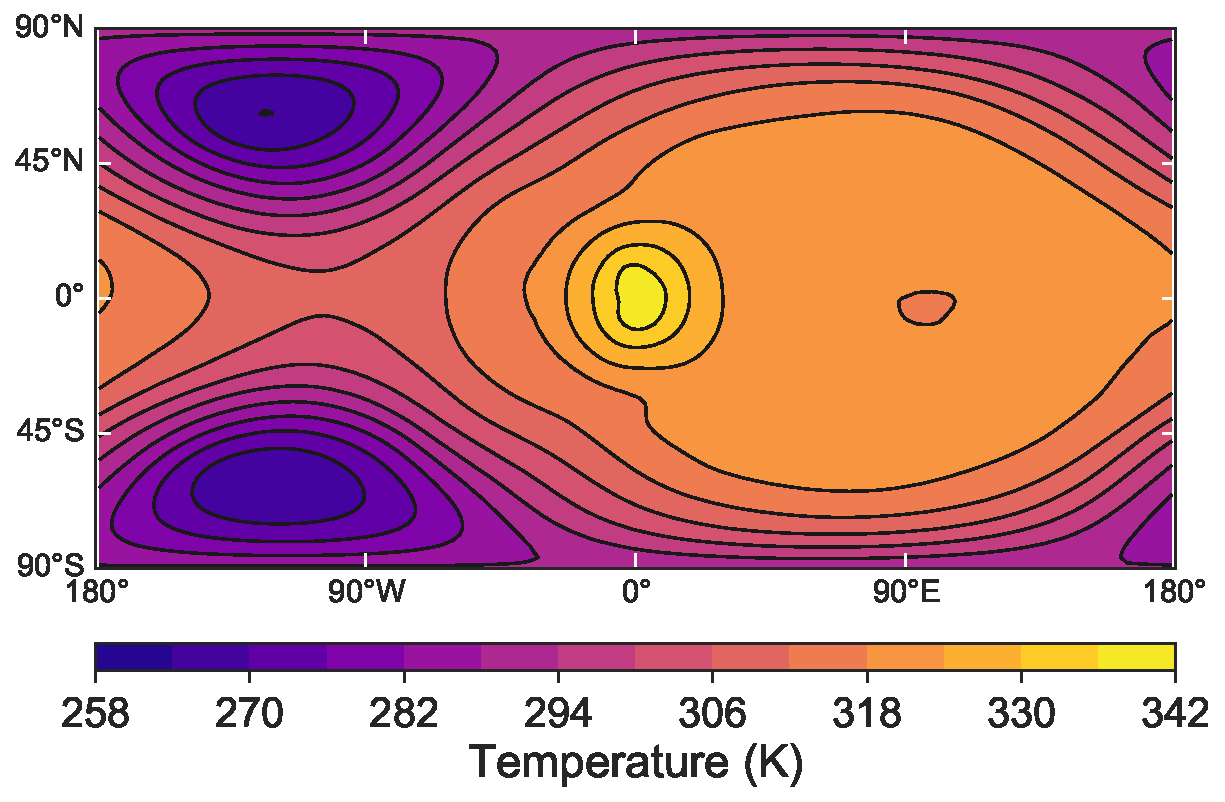
\includegraphics[width=0.65\textwidth]{figures/lit-review/ar_mediumT_10day.pdf}
\caption{The global temperature field at \SI{500}{\milli\bar} of a simulation of a tidally locked Earth-sized planet with a 10 day rotation period and a 1 bar N$_{2}$ atmosphere, showing an eastward shifted hot-spot and night-side cold stationary waves, reproduced from \citet{pierrehumbert2018review}.}\label{fig:review-ar_mediumT_10day}
\end{figure}


The formation of the superrotating jet is still not fully understood. Studies such as \citet{kataria2015atmospheric} compared real observations to the results of GCM simulations of tidally locked hot Jupiters, expecting that the global circulation formed by the GCM was reasonably accurate. However, \citet{thrastarson2010effects} suggested that simulations of the atmospheres of hot Jupiters depended strongly on initial conditions, and that the equilibrium states were not necessarily unique. \citet{liu2013atmospheric} suggested that this was not the case if a bottom drag was applied to the atmosphere, which they justified as an interaction with a deeper layer not represented in the GCM. Their simulations reached the same equilibrium state regardless of the initial conditions. However, \citet{cho2015sensitivity} demonstrated that the short timescale of this drag removed the variability otherwise present in the simulations, and concluded that while a bottom drag may remove sensitivity, it may also remove physically important processes from the atmosphere. \citet{polichtchouk2014intercomparison} further cast doubt on the results of other GCM simulations by showing significant differences between the results of different GCMs modelling the same exoplanets. More recent simulations such as \citet{mendoncca2016thor} have successfully modelled hot Jupiters without applying a bottom drag, suggesting that the earlier discrepancies may have been problems with the specific models. The question of the sensitivity to initial conditions and role of bottom drag is still not fully resolved, which motivates the investigation of the basic dynamics forming this global circulation in Chapter \ref{ch:eqm-zonal-flow}.

It is becoming possible to predict and test scaling relations of atmospheric circulation against observations of many exoplanets in a large parameter space. \citet{komacek2016daynightI}, \citet{komacek2017daynightII}, and \citet{zhang2017dynamics} used a 1D model balancing the advection of heat against radiation to model the circulation of a tidally locked planet. These models were used to explain scaling relations between the observed atmospheric circulation and the bulk composition and parameters of the atmosphere. Chapters \ref{ch:linking-climate-55cnce} and \ref{ch:clouds-lava-planets} will compare simulations of the atmospheric dynamics of the tidally locked planet 55 Cancri to observations of its temperature distribution, to constrain its potential atmospheric properties.












%%%%%%%%%%%%%%%%%%%%%%%%%%%%

%
% % 0 -- LEAD-IN PARAGRAPHS
%
% %START ELEMENT
% Perhaps the most exciting discovery from the field of exoplanet science is that other stars host planets which are very different from those in our solar system. There are similar planets to those in the solar system -- ``hot Jupiters'', high-temperature Jupiter-sized gas giants in short-period orbits, or ``Mini-Neptunes'', which show the literal-mindedness of planetary scientists. But some exoplanets have no analogues in the solar system, and ``lava planets'' are some of the best examples of these.
%
%
% %FRAMING TEXT
% This short chapter describes the class of ``lava planets'', particularly the planet 55 Cancri e, and discusses the question that this thesis aims to answers about this planet.
%
% %SIGNPOSTS
% I will describe lava planets in general, and list the known planets in this class. I will then discuss the 55 Cancri system, and the lava planet 55 Cancri e in that system.
%
% %SUMMARISE CONCLUSIONS
% I will try to show that lava planets are a potentially bountiful area for scientific work, being interesting systems that have observational advantages. I will set up the question of the atmosphere and atmospheric circulation of 55 Cancri e, and show how it relates to the broader question of the nature of the climate of tidally locked planets.
%
%
% %SECTION 1 -- EXOPLANETS
% \section{Exoplanets}
%
% Exoplanets are planets orbiting stars other than our Sun. As far as we know, there is nothing fundamental to distingush the planets in our Solar System from those elsewhere, so it is possible that this specific nomenclature may eventually disappear. I will use the word ``exoplanet''  when discussing specific planets or issues related to their distance, and ``planet'' in a more general or idealised context (such as the first sentence of this paragraph).
%
% There is no better way to date a piece of writing on exoplanets than by announcing how many have been discovered, so I will just note that we know of several thousand and anticipate many more to come. The number of exoplanets which are favourable for detailed observations is still quite small, and we can observe atmospheric details for perhaps only a few dozen planets. In fact, while the title of this thesis suggests it looks at ``lava planets'', there is really only one that is currently observable -- 55 Cancri e. Despite this, I hope to draw general conclusions about the circulation of many types of planet, and contribute to an understanding of tidally locked planets and lava planets for future observations.
%
%
% %SUBSECTION -- DISCOVERY
% \subsection{Discovering Exoplanets}
%
% This is not a thesis on discovering exoplanets, although the methods of discovery are sometimes relevant to the characterisation that is of interest. Most exoplanets discovered to date have been found using either a ``radial velocity`` method or a ``transit'' method.
%
% In the first method, the motion of a star around its common center of mass with a planet orbiting it is detected by measuring the Doppler-shift of emission lines of the star. The magnitude and period of this motion gives the period of the planet's orbit, and a limit on its mass.
%
% In the second method, a planet passing across the line of sight from an observer to the star produces a dip in the light seen by the observer. A periodic dip gives the period of the planet, and the size of the dip gives its radius. So, if a planet can be measured with both methods the observer retrieves its period, mass, radius, density, semi-major axis, and equilibrium temperature.
%
%
% %SUBSECTION -- CHARACTERISATION
% \subsection{Characterising Exoplanets}
%
% This is also not a thesis on characterising exoplanets, although I have tried to keep observations in mind throughout the simulations and theory.
%
% The atmospheres of exoplanets can be characterised through transmission and emission spectroscopy. In transmission spectroscopy, light from the host star passes through the atmosphere of the exoplanet before it reaches the observer, and the spectrum is measured. An alternative (but equivalent) view is that the planet appears to have a different radius as it transits its star at different wavelengths -- at a wavelength the atmosphere is more opaque to, the planet appears larger -- so the absorption spectrum of the gases in the atmosphere can be retrieved.
%
% In emission spectroscopy, the spectrum of the light emitted thermally by the planet and its atmosphere is measured. Hotter planets emit more light in this way, so are better suited to this method.
%
% %SECTION CONCLUSIONS
%
%
%
%
% %SECTION 2 -- LAVA PLANETS
% \section{Lava Planets}
%
% %SUBSECTION --
% \subsection{Tidally Locked Planets}
%
% A tidally locked planet, or a ``synchronously rotating'' planet, always presents the same face to the star it orbits, as its rotation period is the same as its orbital period. An asynchronously rotating planet like the Earth has a different rotation period (1 day) to its orbital period (1 year). Tidal forces slow down the rotation of such planets, until they become tidally locked. The time for a planet to become tidally locked is approximately:
%
%
% See Chapter \ref{ch:wave-mean-flow} for an investigation of the atmospheric dynamics of tidally locked planets.
%
% Tidally locked planets include Hot Jupiters, Earth-like planets like those in the Trappist-1 system, and lava planets like 55 Cancri e, discussed next.
%
% %SUBSECTION --
% \subsection{The Atmospheric Circulation of Tidally Locked Planets}
%
%
%
% %SUBSECTION --
% \subsection{Lava Planets}
%
% ``Lava Planets'' are terrestrial (rocky, not gaseous) planets orbiting very close to their parent star.
%
% %SECTION CONCLUSIONS
%
% %SECTION 3 -- 55 CANCRI E
% \section{55 Cancri e}
%
% 55 Cancri e is a tidally locked lava planet orbiting the binary star 55 Cancri, 41 light years away in the constellation of Cancer.
%
% %SUBSECTION -- 55 Cancri system
% \subsection{The 55 Cancri system}
%
% Figure X shows the 55 Cancri system.
%
% %SUBSECTION -- 55 Cancri e
% \subsection{55 Cancri e}
%
% 55 Cancri e is the closest planet to the G-star 55 Cancri A.
%
% %SUBSECTION -- PHASE CURVE
% \subsection{A Thermal Phase Curve of 55 Cancri e}
%
% A phase curve is the light measured from a planet as it orbits its star. They are particularly useful for tidally locked planets. Figure X shows a phase curve for X.
%
% A thermal phase curve refers to the light emitted by the planet itself, rather than the light it reflects from the star it orbits. For a tidally locked planet, the thermal phase curve shows the hemisphere-averaged brightness temperature of the planet as it rotates.
%
% \citet{demory201655cnce} measured a thermal phase curve of the planet 55 Cancri e.
%
%
%
% %CONCLUSIONS
%
% 55 Cancri e is currently the most easily observable terrestrial tidally locked planet. Its composition, atmosphere, and circulation provide tests of theories of planet formation and atmospheric dynamics. In this thesis, I will use it as a case study for the atmospheric dynamics of tidally locked planets.
%
% %RESTATE SECTION CONCLUSIONS
%
% %OPEN OUT CONCLUSIONS

% \bibliographystyle{unsrtnat}
% \bibliography{../references.bib}
